\documentclass{article}
\usepackage{graphicx}
\usepackage[italian]{babel}
\usepackage[landscape]{geometry}
\usepackage{url}
\usepackage{multicol}
\usepackage{amsmath}
\usepackage{amsfonts}
\pagestyle{empty}
\advance\topmargin-.9in
\advance\textheight2in
\advance\textwidth3.0in
\advance\oddsidemargin-1.45in
\advance\evensidemargin-1.45in
\parindent0pt
\parskip2pt
\newcommand{\hr}{\centerline{\rule{3.5in}{1pt}}}
\begin{document}
\begin{multicols*}{3}
\begin{center}
\textbf{Sage: guida rapida}\\
William Stein (basato su P. Jipsen, trad. F. Zanini)\\
%Latest version at \url{http://wiki.sagemath.org/quickref}\\
GNU Free Document License, estendibile per usi specifici\\
\end{center}
\vspace{-2ex}
\hr\textbf{Notebook}

\includegraphics[width=23em]{nb2}

Calcola cella: $\langle$maiusc-invio$\rangle$

Calcola creando una nuova cella: $\langle$alt-invio$\rangle$

Dividi cella: $\langle$control-;$\rangle$

Unisci celle: $\langle$control-backspace$\rangle$

Inserisci cella matematica: clicca la riga blu tra due celle

Inserisci cella text/HTML: maiusc-clicca la riga blu% tra due celle

Elimina cella: cancella i contenuti e poi backspace

%*********************************************
\hr\textbf{Linea di comando}

\emph{com}$\langle$tab$\rangle$ completa \emph{comando}

*\emph{bar}*? elenca comandi contenenti ``bar''

\emph{comando}\verb|?|$\langle$tab$\rangle$ mostra documentazione

\emph{comando}\verb|??|$\langle$tab$\rangle$ mostra sorgente

\verb|a.|$\langle$tab$\rangle$ mostra metodi dell'oggetto \verb|a| \quad
(di più: \verb|dir(a)|)

\verb|a._|$\langle$tab$\rangle$ mostra metodi nascosti dell'oggetto \verb|a| \quad

\verb|search_doc("|\emph{stringa o regexp}\verb|")| \quad ricerca nella doc.

\verb|search_src("|\emph{stringa o regexp}\verb|")| \quad ricerca codice sorgente

\verb|_| è l'output precedente

%*********************************************
\hr\textbf{Numeri}

Interi: $\mathbf Z=$ \verb|ZZ | es. \verb|-2  -1  0  1  10^100|

Razionali: $\mathbf Q=$ \verb|QQ | es. \verb|1/2  1/1000  314/100  -2/1|

Reali: $\mathbf R\approx$ \verb|RR | es. \verb|.5  0.001  3.14  1.23e10000|

Complessi: $\mathbf C\approx$ \verb|CC | es. \verb|CC(1,1)  CC(2.5,-3)|

Precisione doppia: \verb|RDF| and \verb|CDF | es. \verb|CDF(2.1,3)|

Mod $n$: $\mathbf Z/n\mathbf Z = $ \verb|Zmod | es. \verb|Mod(2,3)   Zmod(3)(2)|

Campi finiti: $\mathbf F_q=$ \verb|GF | es. \verb|GF(3)(2)   GF(9,"a").0|

Polinomi: $R[x,y]$ es. \verb|S.<x,y>=QQ[]   x+2*y^3|

Serie: $R[[t]]$ es. \verb|S.<t>=QQ[[]]    1/2+2*t+O(t^2)|

Numeri $p$-adici: $\mathbf Z_p\approx$\verb|Zp|, $\mathbf Q_p\approx$\verb|Qp| es. \verb| 2+3*5+O(5^2)|

Chiusura algebrica: $\overline{\mathbf Q} = $ \verb|QQbar| es. \verb|QQbar(2^(1/5))|

Aritmetica degli intervalli: \verb| RIF | es. \verb|RIF((1,1.001))|

Campo di numeri: \verb|R.<x>=QQ[];K.<a>=NumberField(x^3)|


%*********************************************
 \hr\textbf{Aritmetica}

$ab=$ \verb|a*b| \quad $\frac a b=$ \verb|a/b| 
\quad 
$a^b=$ \verb|a^b| \quad $\sqrt{x}=$ \verb|sqrt(x)|

$\sqrt[n]{x}=$ \verb|x^(1/n)|
\quad 
$|x|=$ \verb|abs(x)|
\quad 
$\log_b(x)=$ \verb|log(x,b)|

Somme:
$\displaystyle\sum_{i=k}^n f(i)=$ \verb|sum(f(i) for i in (k..n))|

Prodotti:
$\displaystyle\prod_{i=k}^n f(i)=$ \verb|prod(f(i) for i in (k..n))|


%*********************************************
 \hr\textbf{Costanti e funzioni}

Costanti: $\pi=$ \verb|pi| \quad $e=$ \verb|e| \quad $i=$ \verb|i| 
\quad $\infty=$ \verb|oo| 

$\phi=$ \verb|golden_ratio| \quad $\gamma=$ \verb|euler_gamma|

Approssima: \verb|pi.n(digits=18)| $=3.14159265358979324$

Funzioni: \verb|sin cos tan sec csc cot sinh cosh tanh| \verb|sech csch coth log ln exp| ...

Funzioni Python: \verb| def f(x): return x^2|

%*********************************************
\hr\textbf{Funzioni interattive}

Metti \verb|@interact| prima della funzione

\verb|@interact|

\verb|def f(n=[0..4], s=(1..5), c=Color("red")):|

\verb|  var("x");show(plot(sin(n+x^s),-pi,pi,color=c))|

%*********************************************
\hr\textbf{Espressioni simboliche}

Definisci nuove variabili simboliche: \verb|var("t u v y z")|

Funzioni simboliche: es. $f(x)=x^2$ \qquad \verb| f(x)=x^2|

Relazioni: \verb|f==g  f<=g  f>=g  f<g  f>g|

Risolvi $f=g$: \verb| solve(f(x)==g(x), x)|

\verb|            solve([f(x,y)==0, g(x,y)==0], x,y)|

\verb|factor(...)|\qquad \verb|expand(...)|\qquad \verb|(...).simplify_...|

\verb|find_root(f(x), a, b)|\quad trova $x\in [a,b]$ s.t. $f(x)\approx 0$

%*********************************************
\hr\textbf{Analisi}

$\displaystyle\lim_{x\to a} f(x)=$ \verb|limit(f(x), x=a)|

$\frac{d}{dx}(f(x))=$ \verb|diff(f(x),x)|

$\frac{\partial}{\partial x}(f(x,y))=$ \verb|diff(f(x,y),x)|

\verb|diff| $=$ \verb|differentiate| $=$ \verb|derivative|

$\int f(x)dx=$ \verb|integral(f(x),x)|

$\int_a^b f(x)dx=$ \verb|integral(f(x),x,a,b)|

$\int_a^b f(x)dx \approx$ \verb|numerical_integral(f(x),a,b)|

Polinomio di Taylor, grado $n$ in $a$: \texttt{taylor(f(x),x,$a$,$n$)} 


%*********************************************
\hr\textbf{Grafici 2D}

\includegraphics[width=12em]{2d}

\texttt{line([($x_1$,$y_1$),$\ldots$,($x_n$,$y_n$)],$\it opzioni$)}

\texttt{polygon([($x_1$,$y_1$),$\ldots$,($x_n$,$y_n$)],$\it opzioni$)}

\texttt{circle(($x$,$y$),$r$,$\it opzioni$)}

\texttt{text("txt",($x$,$y$),$\it opzioni$)}

\emph{opzioni} come in \verb|plot.options|, 
es. \texttt{thickness=$\it pixel$},

\texttt{rgbcolor=($r$,$g$,$b$)},
\quad \texttt{hue=$h$} \quad dove $0\le r,b,g,h\le 1$

\texttt{show({\it grafico}, {\it opzioni})}

\verb|figsize=[w,h]| per cambiare le dimensioni

\verb|aspect_ratio=|{\it numero} per cambiare le proporzioni


\texttt{plot(f($x$),$(x, x_{\rm min}, x_{\rm max})$,$\it options$)}

\texttt{parametric\_plot((f($t$),g($t$)),$(t, t_{\rm min}, t_{\rm max})$,$\it options$)}

\texttt{polar\_plot(f($t$),$(t, t_{\rm min}, t_{\rm max})$,$\it opzioni$)}

combina: \verb|circle((1,1),1)+line([(0,0),(2,2)])|

\texttt{animate(}\emph{elenco di grafici, opzioni}\texttt{).show(delay=20)}

%*********************************************
\hr\textbf{Grafici 3D}
 
\includegraphics[width=15em,height=8em]{3d}

\texttt{line3d([($x_1$,$y_1$,$z_1$),$\ldots$,($x_n$,$y_n$,$z_n$)],$\it opzioni$)}

\texttt{sphere(($x$,$y$,$z$),$r$,$\it opzioni$)}

\texttt{text3d("txt", ($x$,$y$,$z$), $\it opzioni$)}

\texttt{tetrahedron(($x$,$y$,$z$),$dimensione$,$\it opzioni$)}

\texttt{cube(($x$,$y$,$z$),$dimensione$,$\it opzioni$)}

\texttt{octahedron(($x$,$y$,$z$),$dimensione$,$\it opzioni$)}

\texttt{dodecahedron(($x$,$y$,$z$),$dimensione$,$\it opzioni$)}

\texttt{icosahedron(($x$,$y$,$z$),$dimensione$,$\it opzioni$)}

\texttt{plot3d(f($x,y$),$(x,x_{\rm b},x_{\rm e})$, $(y,y_{\rm b},y_{\rm e})$,$\it opzioni$)}

\texttt{parametric\_plot3d((f,g,h),$(t, t_{\rm b}, t_{\rm e})$,$\it opzioni$)}

\texttt{parametric\_plot3d((f($u,v$),g($u,v$),h($u,v$)),}

\qquad \qquad \qquad \qquad 
\texttt{$(u,u_{\rm b},u_{\rm e})$,$(v,v_{\rm b},v_{\rm e})$,$\it opzioni$)}

\emph{opzioni}: \texttt{aspect\_ratio=$[1,1,1]$, color="red"} 

\texttt{opacity=0.5, figsize=6, viewer="tachyon"}

%*********************************************
\hr\textbf{Matematica discreta}

$\lfloor x\rfloor=$ \verb|floor(x)| 
\quad 
$\lceil x\rceil=$ \verb|ceil(x)|

Resto di $n$ diviso per $k=$ \verb|n%k| \quad\, $k|n$ sse \verb| n%k==0|

$n!=$ \verb|factorial(n)| \qquad
${x\choose m}=$ \verb|binomial(x,m)|

$\phi(n)=$ \texttt{euler\_phi($n$)}

Stringhe: es. \ \verb|s = "Ciao"| = \verb|"Ci"+'ao'|

\texttt{s[0]="C" \quad s[-1]="o" \quad s[1:3]="ia" \quad s[2:]="ao"}

Elenchi: es. \ \verb|[1,"Ciao",x]| = \verb|[]+[1,"Ciao"]+[x]|

Tuple: es. \ \verb|(1,"Ciao",x)| \quad (immutabile)

Insiemi: es. \ $\{1,2,1,a\}=$ \verb|Set([1,2,1,"a"])|

Comprensione elenchi $\approx$ notazione costruttore insiemi, es.

$\{f(x):x\in X, x>0\}=$ \verb|Set([f(x) for x in X if x>0])|

 
%*********************************************
\hr\textbf{Teoria dei grafi}

\includegraphics[width=6em]{graph}  

Grafo: \texttt{G = Graph(\{0:[1,2,3], 2:[4]\})}

Grafo orientato: \texttt{DiGraph({\it dictionary})}

Famiglie di grafici: \texttt{graphs.}$\langle$tab$\rangle$  

Invarianti: \texttt{G.chromatic\_polynomial()}, \texttt{G.is\_planar()}

Cammini: \texttt{G.shortest\_path()}

Visualizza: \texttt{G.plot()}, \texttt{G.plot3d()}

Automorfismi: \texttt{G.automorphism\_group()},

\texttt{G1.is\_isomorphic(G2)}, \texttt{G1.is\_subgraph(G2)}


%*********************************************
\hr\textbf{Calcolo combinatorio}

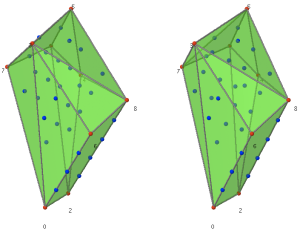
\includegraphics[width=8em]{polytope.png}

Sequenze di interi: \texttt{sloane\_find({\it list})}, \texttt{sloane.}$\langle$tab$\rangle$  

Partizioni:
\texttt{P=Partitions({\it n})}\quad \texttt{P.count()}

Combinazioni: \texttt{C=Combinations({\it list})}\quad\texttt{C.list()}

Prodotto cartesiano: \texttt{CartesianProduct(P,C)}

Tabelle: \texttt{Tableau([[1,2,3],[4,5]])}

Parole: \texttt{W=Words("abc"); W("aabca")}

Ordinamenti parziali: \texttt{Poset([[1,2],[4],[3],[4],[]])}

Sistemi di radici: \texttt{RootSystem(["A",3])}

Cristalli: \texttt{CrystalOfTableaux(["A",3], shape=[3,2])}

Politopi reticolari: \verb|A=random_matrix(ZZ,3,6,x=7)|

\verb|L=LatticePolytope(A)    L.npoints()   L.plot3d()|

%*********************************************
\hr\textbf{Algebra di matrici}

$\begin{pmatrix}1\\2\end{pmatrix}=$ \verb|vector([1,2])|

$\begin{pmatrix}1&2\\3&4\end{pmatrix}=$ \verb|matrix(QQ,[[1,2],[3,4]], sparse=False)|

$\begin{pmatrix}1&2&3\\4&5&6\end{pmatrix}=$ \verb|matrix(QQ,2,3,[1,2,3, 4,5,6])|

$\left|\begin{matrix}1&2\\3&4\end{matrix}\right|=$
\verb|det(matrix(QQ,[[1,2],[3,4]]))|

$Av=$ \verb|A*v| \quad $A^{-1}=$ \verb|A^-1| \quad $A^t=$ \verb|A.transpose()|

Risolvi $Ax=v$: \verb| A\v  | or \verb| A.solve_right(v)|

Risolvi $xA=v$: \verb| A.solve_left(v)|

Forma triangolare superiore: \verb| A.echelon_form()|

Rango e nullità: \verb|A.rank()    A.nullity()|

Forma di Hessenberg: \verb|A.hessenberg_form()|

Polinomio caratteristico: \verb|A.charpoly()|

Autovalori: \verb|A.eigenvalues()| 

Autovettori: \verb|A.eigenvectors_right()| (also left)

Gram-Schmidt: \verb|A.gram_schmidt()|

Visualizza: \verb|A.plot()|

Riduzione LLL: \verb|matrix(ZZ,...).LLL()|

Forma di Hermite: \verb|matrix(ZZ,...).hermite_form()|

%*********************************************
\hr\textbf{Algebra lineare}

\includegraphics[width=12em,height=6em]{linalg}

Spazio vettoriale $K^n = $ \verb| K^n | e.g. \verb| QQ^3   RR^2   CC^4|

Sottospazio: \verb|span(vectors, |{\it field}\verb| )|, es.

\verb|span([[1,2,3], [2,3,5]], QQ)|

Nucleo: \verb|A.right_kernel()| (anche sinistro)

Somma e intersezione: \verb|V + W | e \verb| V.intersection(W)|

Base: \verb|V.basis()|

Matrice di base: \verb|V.basis_matrix()|

Restringi matrice a un sottospazio: \texttt{A.restrict(V)}

Vettore scritto su una base: \texttt{V.coordinates({\it vector})}

%*********************************************
\hr\textbf{Matematica numerica}

Pacchetti: \verb|import numpy, scipy, cvxopt|

Minimizzazione: \verb|var("x y z")|

\verb|   minimize(x^2+x*y^3+(1-z)^2-1, [1,1,1])|


%*********************************************
\hr\textbf{Teoria dei numeri}

Primi: \verb|prime_range(n,m)|, \verb|is_prime|, \verb|next_prime|

Fattorizza: \verb|factor(n)|, \verb|qsieve(n)|, \verb|ecm.factor(n)|

Simbolo di Kronecker: $\left(\frac{a}{b}\right) = $ \texttt{kronecker\_symbol({\it a},{\it b})}

Frazioni continue: \verb|continued_fraction(x)|

Numeri di Bernoulli: \texttt{bernoulli(n)}, \texttt{bernoulli\_mod\_p(p)}

Curve ellittiche: \verb|EllipticCurve([|$a_1,a_2,a_3,a_4,a_6$\verb|])|

Caratteri di Dirichlet: \texttt{DirichletGroup({\it N})}

%Congruence subgroups: \texttt{Gamma0({\it N})}, \texttt{Gamma1({\it N})}, \texttt{GammaH}

Forme modulari: \texttt{ModularForms({\it level}, {\it weight})}

Simboli modulari: \texttt{ModularSymbols({\it level}, {\it weight}, {\it sign})}

Moduli di Brandt: \texttt{BrandtModule({\it level}, {\it weight})}

Varietà modulari Abeliane: \texttt{J0({\it N})}, \texttt{J1({\it N})}

%*********************************************
\hr\textbf{Teoria dei gruppi}

\texttt{G = PermutationGroup([[(1,2,3),(4,5)],[(3,4)]])}

\texttt{SymmetricGroup({\it n})}, \texttt{AlternatingGroup({\it n})} 

Gruppi abeliani: \texttt{AbelianGroup([3,15])}

Gruppi di matrici: \texttt{GL, SL, Sp, SU, GU, SO, GO}

Funzioni: \texttt{G.sylow\_subgroup(p)}, \texttt{G.character\_table()}, 

\texttt{G.normal\_subgroups()}, \texttt{G.cayley\_graph()}


%*********************************************
\hr\textbf{Anelli non commutativi}

Quaternioni: \texttt{Q.<i,j,k> = QuaternionAlgebra(a,b)}

Algebra libera: \texttt{R.<a,b,c> = FreeAlgebra(QQ, 3)}

%Steenrod algebra: \texttt{SteenrodAlgebra({\it prime})}

%*********************************************
\hr\textbf{Moduli Python}

\verb|import| \emph{nome\_del\_modulo}

\verb|module_name.|$\langle$tab$\rangle$ e \verb|help(module_name)|

%\verb|sage.|\emph{module\_name}\verb|.all.|$\langle$tab$\rangle$ mostra i comandi esportati

%\mbox{Pacchetti standard: Maxima GP/PARI GAP Singular R Shell ...}

%Pacchetti opzionali: Biopython Gnuplot Kash ...

%\%\emph{nome\_del\_pacchetto} poi usa la sintassi del comando

%*********************************************
\hr\textbf{Personalizzazione e debugging}

\verb|time| \emph{comando}: \quad  mostra informazioni di timing

\verb|timeit("comando")|: misura il tempo del comando

\verb|t = cputime(); cputime(t)|: tempo CPU trascorso

\verb|t = walltime(); walltime(t)|: tempo reale trascorso

\verb|%pdb|: attiva debugger interattivo (solo linea di comando)

\verb|%prun comando|: personalizza comando (solo ldc)

\end{multicols*}

\end{document}
